\chapter{Methodology}\label{chapter:Methodology}
\section{Research Design}
Based on our extensive literature review, we pursue a quantitative research approach to test the hypotheses against empirical data. Two distinct regression designs are applied: A linear regression model is used to test the hypothesis concerning research question one. In this model, the three latent variables of Ajzen's TPB are exogenous variables predicting the EI. For research question two, we provide evidence by means of a mediation analysis based on \cite{baron1986moderator}.
To gather the relevant data, we are using a structured questionnaire. The validated, multi-item questionnaire is assessed via a seven-point Likert scale and is administered once with students from technical study programs at the Technical University Munich. The survey assesses four latent variables: personal attitude, subjective norm, perceived behavioral control and the level of EI.  Furthermore, we assess whether students have participated in a university course for developing a technical prototype. We also include questions to assess five control variables: Degree program, study subject, total number of semesters, gender and country of birth.

\section{Data Collection}

The gathered and cleaned information as well as the regression analysis and outcomes are publicly available at: 

\begin{center}
\textit{https://github.com/lukasmohs/entrepreneurial-intention-analysis}
\end{center} 

see print version of our survey in appendi

\section{Variables}
\section{Sample}
\section{Regression Models}

Refer to symbols or abbreviations with\\\verb+\gls{symbolname} \glstext{symbolname} \glsfirst{symbolname}+:\\
\gls{symb:N} \glstext{symb:N} \glsfirst{symb:N}\\
\gls{BA} \gls{DA} \gls{MA}

Refer to other sections with \verb+\ref{labelname}+:\\
A reference to this subsection: \ref{labelname}

Include figures with\\
\verb+\begin{figure}+\\
\verb+...+\\
\verb+\caption{An example figure}\label{fig:example}\end{figure}+

\begin{figure}[h]
\begin{center}
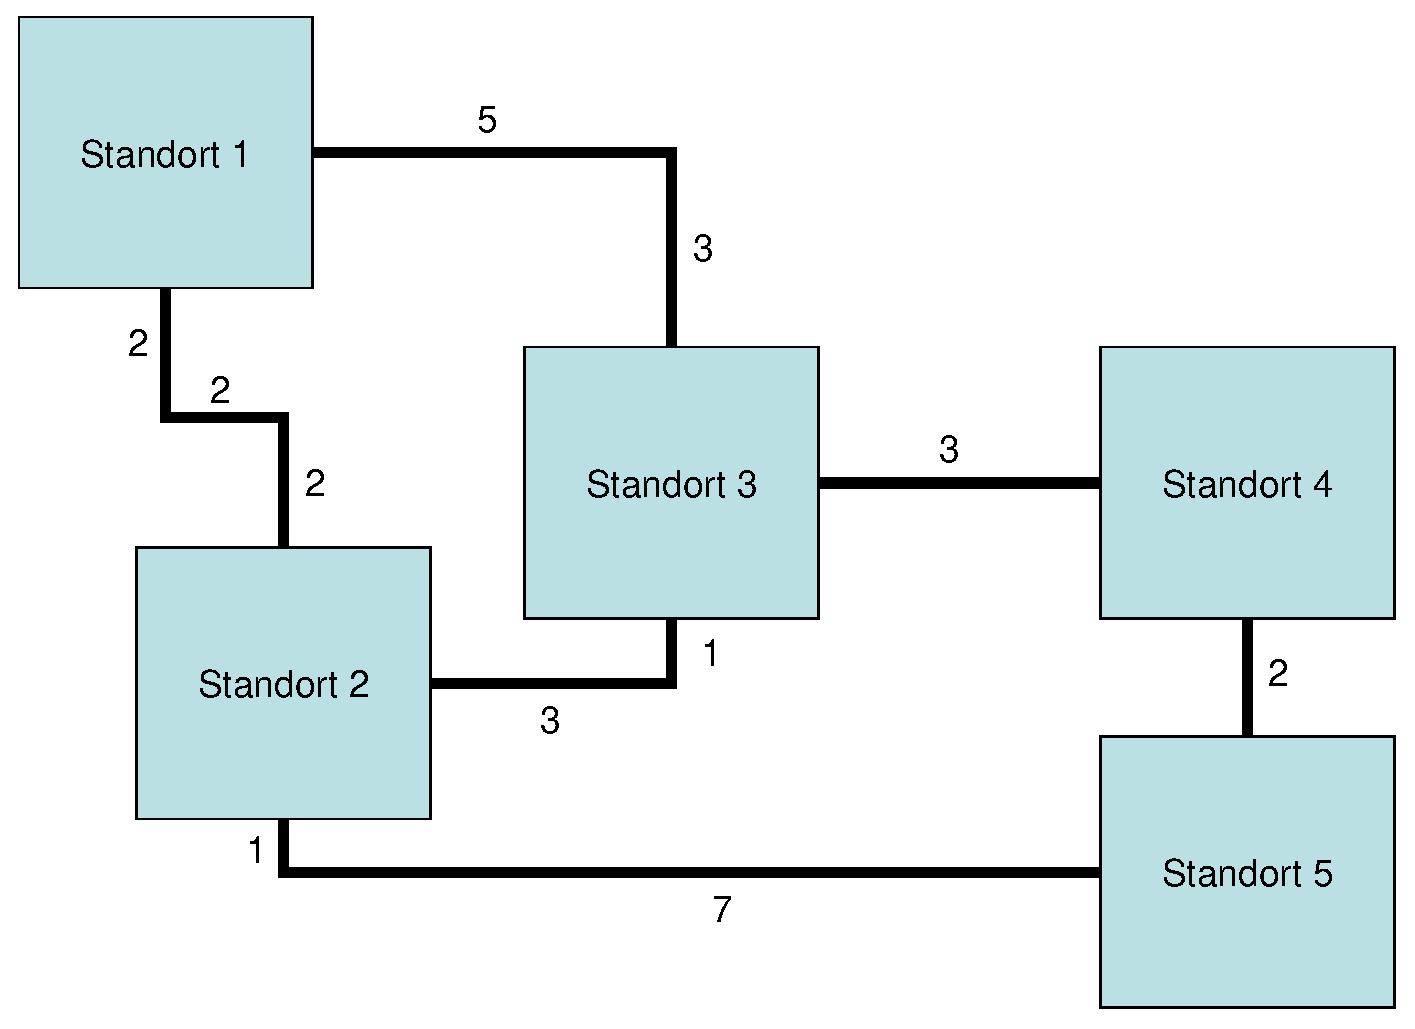
\includegraphics[width=10cm]{images/example_figure}
\caption{An example figure}
\label{fig:example}
\end{center}
\end{figure}

Include only PostScript images (.eps) if you want to create a PostScript document using dvips and only .pdf, .png, .jpeg and .gif images if your goal is a PDF document using pdflatex.